%!TEX option=--shell-escape
\documentclass[journal]{IEEEtran}
\usepackage{minted}
\usepackage{dirtree}
\usepackage{subfig}
\usepackage{tikz}
\usepackage{amsmath,bm,times}
\usepackage{pstricks}
\usepackage{graphicx}
\usepackage{underscore}
\newcommand{\mx}[1]{\mathbf{\bm{#1}}} % Matrix command
\newcommand{\vc}[1]{\mathbf{\bm{#1}}} % Vector command
\usemintedstyle{tango}
\title{Contributor's Guide SRT}
\author{Vidhyashree Nagaraju, Karthik, Lance Fiondella }

\begin{document}
\maketitle

\section{Introduction}

SRT is a tool to determine and estimate the reliability of a software by analysing the failure data. The analysis of data is done by different reliability models. The failure data could be of failure rate form or failure count form. The tool should adapt to the format presented to it and run models on the given data. The best fit model is choosen the end user. Software reliability is important for mission critical systems the models should represent the data as closely as possible. The conventional way to achieve more reliable estimates is to run differend models on the given data and choose the best based on the GOF (Goodness of Fit measures). More models more choice and better prediction of software reliability. The tools available now to estimate the software are closed source. This is not just an attempt to design an open-source tool but a framework for researchers to contribute their own.


\section{Model Architecture}
The model folder structure is as follows:

\dirtree{%
.1 SRT.
.2 models.
.3 model-1.
.4 model-1-implementation.R.
.3 model-2.
.3 model-3.
.2 modelspecifications.R.
}

\section{Simplified Architecture}

The actual Implementation is simplified in the below diagram to let the contributors focus on the model implementation. You can skip the details but its good to know the implementation details if you have to use an unconventional approach to implement your model.

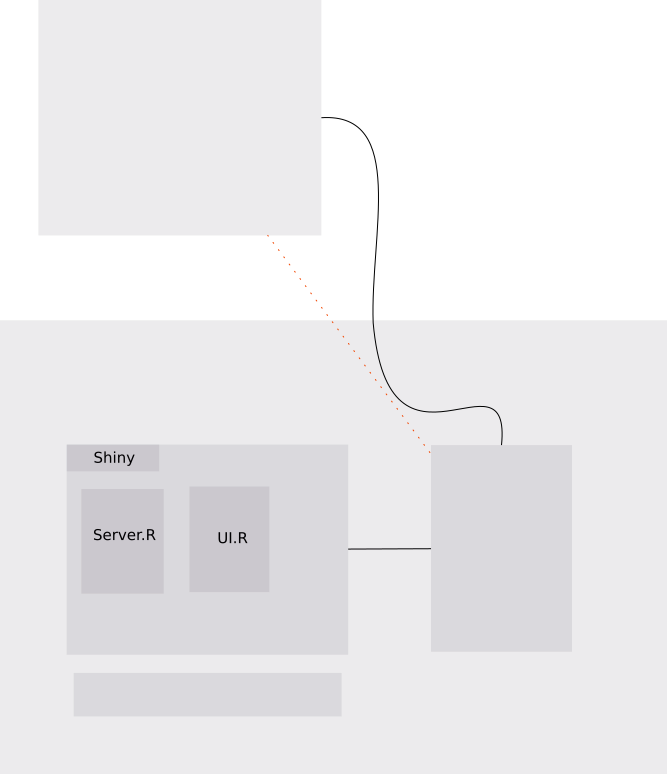
\includegraphics[scale=0.35]{../document.png}


\section{Model Specifications}

Model specification provide additional details about the model. The contributors can in detail......


Example model specifications:



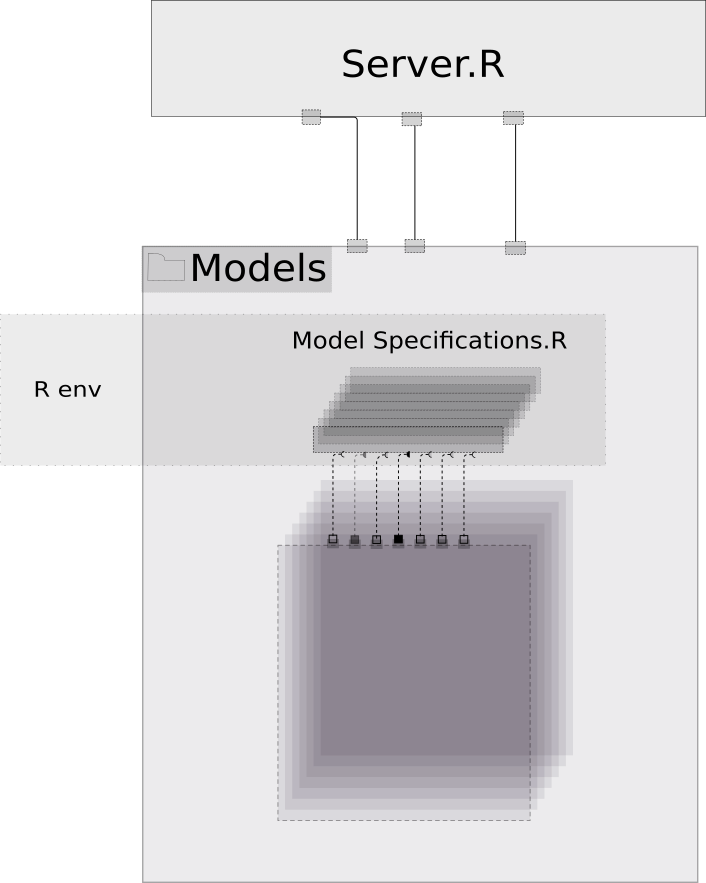
\includegraphics[scale=0.35]{../ModelSpecifications.png}
\begin{minted}[numbersep=1pt,
               gobble=0,
               frame=lines,
               framesep=2mm,
               fontfamily=courier]{R}
  # Jelinksi-Moranda Model
  JM_input        <- c("IF")
  JM_methods      <- c("BM")
  JM_params       <- c("N0","Phi")
  JM_numfailsparm <- c(1)
  JM_fullname   <- c("Jelinski-Moranda")
  JM_plotcolor  <- c("red")
  JM_type       <- c("FR","Exp")
  JM_Finite     <- TRUE
  JM_Results    <- data.frame(
  		"format"="xlsx",
		  "fileName"="model_data")
\end{minted}

The model can take data vector of Failure times 'FT', Inter failures times 'IF', failure count 'FC'. So the input vector type for a given model should be specified. For Jelinksi model defined above default input vector is defined as Inter-Failure Times ('IF'). The model could implement any algorithm to find the parameters. The mumerical method algorithms were kept in mind while designing the tool but bayesian methods can also be used for parameters estimation. The Jelinksi here is using Bisection method. The short form is strongly encouraged but not mandatory as long as you follow the guidelines. The parameters of a model should be defined in 'JM_params' variable. The Model specific funtion '{model}_MLE({args})' [ex: JM_BM_MLE() ] should return the estimated parameters with labels as defined in the JM_params so that the repective parameters will be called as required without knowledge of the model being used. JM_numfailsparm............................. {MODEL}_fullname variable will used by the user interface end to list the available models. Full names will be user friendly. JM_plotcolor is used to specify the color user should expect in the plots [ Note: this is disabled temporarily and will functional pretty soon] . {MODEL}_type is an experimental feature which is not funtional/implemented but its potential use is to categorize the type of models based on data. Any machine learning algorithm could be used to categorize the data and might depend on the labels for categorization. The {MODEL}_Finite is to define if the model is Finite type or not. Its a boolean type variable and expects only TRUE or FALSE as parameters. Note that TRUE and FALSE are datatypes and "TRUE" in quotes is not equivalent to TRUE.  The model results variable should the point to the results filename. The models which the users contribute should pass the test on the standard data sets provided by Handbook of Software reliability. The pass or fail of a test is based on the tolerance error and time it takes to evaluate. The model specifications is key to the contribution. With increasing contributions from different sources the manual way of checking the model could turn cumbersome and time taking process. To avoid that we intend to use the continuous integration tool to check the model against the results. At that point the users will not be able to integrate thier model untill they could get through the test.  

\end{document}